\chapter{Giới thiệu các hàm kích hoạt được sử dụng}\label{chap:gioithieucachamkichhoatduocsudung}

\section{Những yêu cầu tối thiểu của hàm kích hoạt trong mạng học sâu}\label{sec:nhungyeucauvavande}

Những hàm kích hoạt được giới thiệu đều là những hàm kích hoạt phi tuyến.
Lý do hàm kích hoạt không được phép là một hàm tuyến tính có thể nhìn ở nhiều góc độ.
Nếu ta sử dụng các hàm kích hoạt tại một tầng ẩn nào đó là một hàm tuyến tính, tầng này và tầng tiếp theo có thể rút gọn thành một tầng.
Vì hợp của các hàm tuyến tính là một hàm tuyến tính.
Giả sử ta có một mạng nơ-ron chỉ gồm 2 tầng ẩn đều sử dụng hàm kích hoạt là một hàm tuyến tính $f(\mathbf{x}) = \mathbf{x}$.
Ta dễ dàng suy ra được như sau:
\begin{align}
    \mathbf{a}^{(1)} &= f\left(\mathbf{z}^{(1)}\right) = f\left(\mathbf{W}^{(1)}x + \mathbf{b}^{(1)}\right) = \mathbf{W}^{(1)}x + \mathbf{b}^{(1)} \nonumber\\
    \mathbf{a}^{(2)} &= f\left(\mathbf{z}^{(2)}\right) = f\left(\mathbf{W}^{(2)}\mathbf{a}^{(1)} + \mathbf{b}^{(2)}\right) \nonumber\\
    &= f\left(\mathbf{W}^{(2)}\left(\mathbf{W}^{(1)}\mathbf{x} + \mathbf{b}^{(1)}\right) + \mathbf{b}^{(2)}\right) \nonumber\\
    &= f\left(\underbrace{\mathbf{W}^{(2)}\mathbf{W}^{(1)}}_{\mathbf{W}^*}\mathbf{x} + \underbrace{\mathbf{W}^{(2)}\mathbf{b}^{(1)} + \mathbf{b}^{(2)}}_{\mathbf{b}^*}\right) \nonumber\\
    &= f\left(\mathbf{W}^*\mathbf{x} + \mathbf{b}^*\right) = \mathbf{W}^*\mathbf{x} + \mathbf{b}^* \label{eqn:tohopcuax}
\end{align}

\begin{figure}[!h]
\captionsetup{width=0.8\textwidth}
\centering
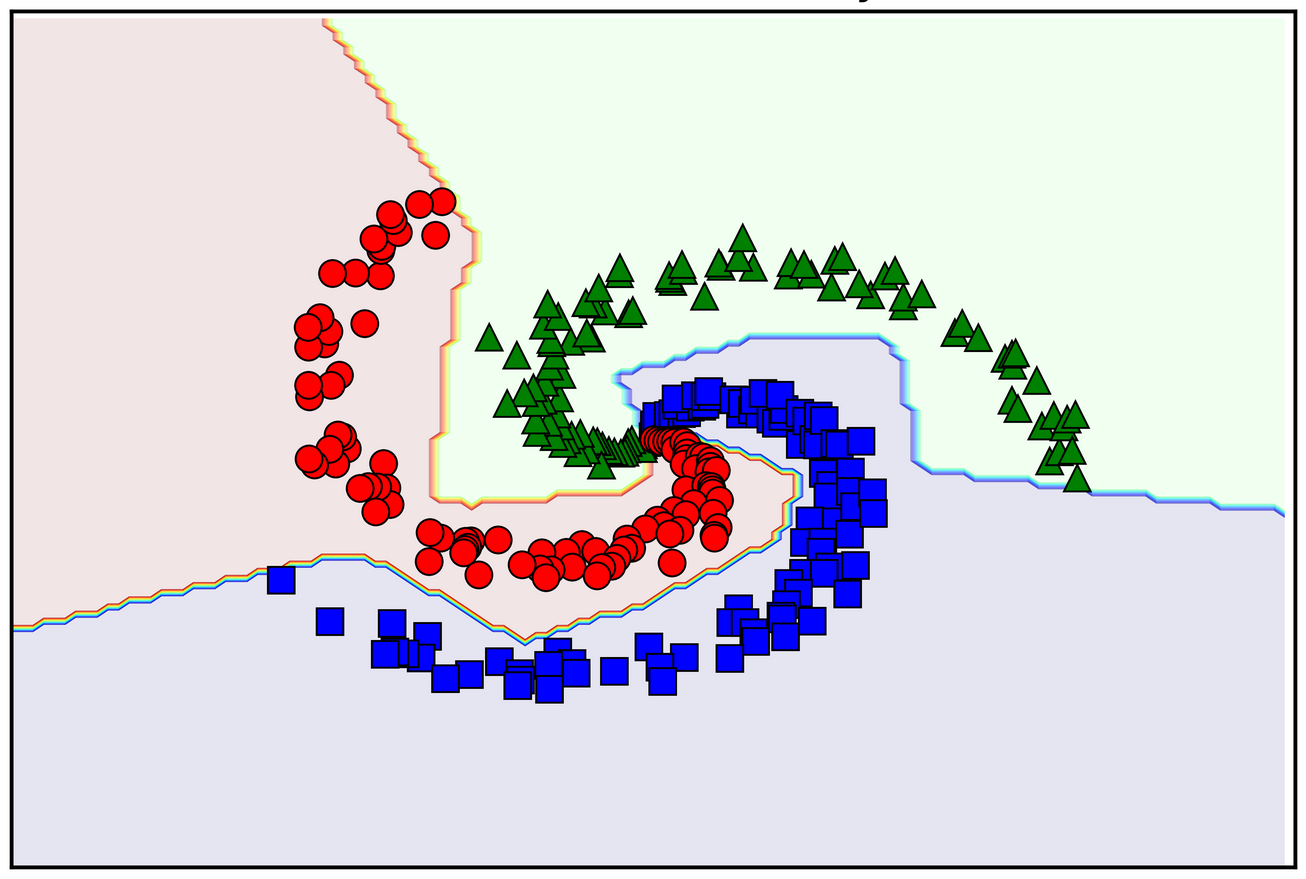
\includegraphics[width=10cm]{images/nonlinearland.PNG}
\caption{Phân lớp các dữ liệu sử dụng những miền phi tuyến tính \cite{mlpvuhuutiep}.}
\label{fig:nonlinearland}
\end{figure}

Theo như \ref{eqn:tohopcuax} thì đầu ra của tầng ẩn thứ 2 vẫn chỉ là một tổ hợp tuyến tính của $\mathbf{x}$ ban đầu.
Thế thì khi một mạng nơ-ron sâu có tất cả các tầng ẩn đều sử dụng những hàm kích hoạt tuyến tính, ta có thể rút gọn những tầng ẩn này đi mà chỉ có tầng đầu vào và tầng đầu ra.
Điều này làm cho mô hình không thể hiện được tính sâu, thứ làm nên sức mạnh của những mạng nơ-ron.
\vspace{5pt}

Ở một góc nhìn đơn giản, bản thân những hàm tuyến tính chỉ có thể làm việc được với những bài toán đơn giản.
Nếu chỉ sử dụng những hàm kích hoạt tuyến tính thì ta cũng chỉ có thể đa ra một lời giải đơn giản.
Mà rõ ràng, những bài toán được áp dụng trong mạng học sâu không chỉ có những bài toán đơn giản mà còn là những bài toán rất phức tạp.
Những hàm tuyến tính không thể nào đáp ứng được nhu cầu bài toán đưa ra, chẳng hạn như hình \ref{fig:nonlinearland}, nếu chỉ dùng những hàm tuyến tính để phân lớp thì ta sẽ không bao giờ có một lời giải tốt.
Do đó, hàm kích hoạt được yêu cầu phải là một hàm phi tuyến.
\vspace{5pt}

Nền móng của mạng nơ-ron sâu là mô hình perceptron \cite{luocsudlvuhuutiep}, với hàm kích hoạt được sử dụng là hàm dấu.
\begin{align}
    \text{sgn}(x) = \begin{cases}-1, &x < 0\\ 0, &x = 0\\ 1, &x > 0\end{cases}
\end{align}

Dù rằng là hàm này phi tuyến, nhưng thực tế lại không được sử dụng, vì đạo hàm tại hầu hết các điểm bằng 0 (trừ tại gốc toạ độ không có đạo hàm).
Việc đạo hàm bằng 0 này khiến cho các thuật toán dựa trên gradient không hoạt động.
Trong khi việc tối ưu các mạng học sâu sử dụng lan truyền ngược lại dựa trên gradient.

\section{Hàm Sigmoid và hàm Tanh}\label{sec:hamsigmoidvahamtanh}

Hàm Sigmoid, hay còn biết đến với cái tên là hàm logistic. Hàm được định nghĩa toán học như sau:
\begin{align}
    \text{Sigmoid}(x) = \sigma(x) = \dfrac{1}{1 + e^{-x}}
\end{align}

\begin{figure}[!h]
\captionsetup{width=0.8\textwidth}
\centering
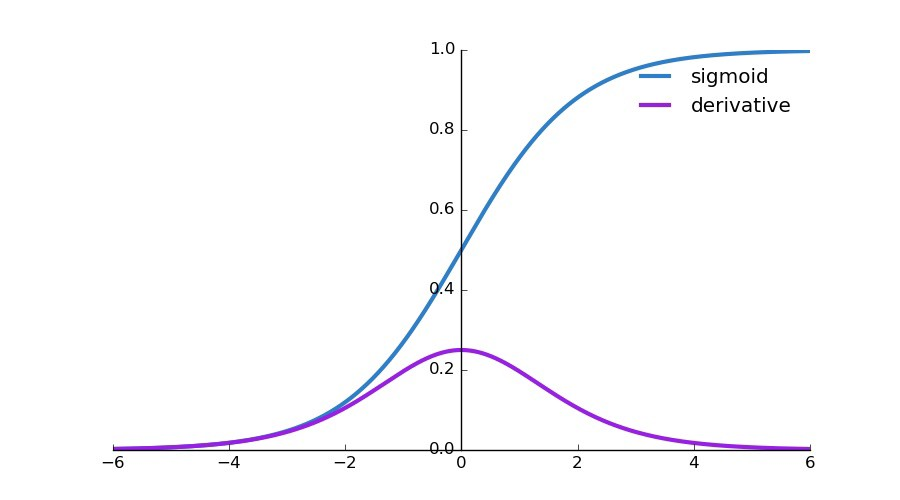
\includegraphics[width=15cm]{images/sigmoidfunc.jpg}
\caption{Đồ thị hàm số của hàm Sigmoid và đạo hàm của nó.}
\label{fig:sigmoidfunc}
\end{figure}

Nhìn vào \ref{fig:sigmoidfunc} ta thầy rằng: nếu đầu vào lớn, hàm số sẽ cho đầu ra gần với 1;
nếu đầu vào nhỏ (rất âm), hàm số sẽ cho đầu ra gần với 0.
Trước đây, hàm kích hoạt này được sử dụng rất nhiều vì có đạo hàm rất đẹp (xem hình \ref{fig:sigmoidfunc}).
Nhưng những năm gần đây, hàm số này ít khi được sử dụng để làm hàm kích hoạt cho các tầng ẩn.
Thay vào đó, hàm Sigmoi được sử dụng ở tầng đầu ra khi đầu ra là các giá trị nhị phân hoặc biểu diễn các xác suất.
\vspace{5pt}

Một hàm tương tự thường sử dụng và mang lại hiệu quả tốt hơn chính là hàm Tanh:
\begin{align}
    \tanh{x} = \dfrac{e^x - e^{-x}}{e^x + e^{-x}}
\end{align}

Hàm số này có tính chất đầu ra chạy từ -1 đến 1, khiến cho nó có tính chất tâm 0 thay vì chỉ dương như hàm Sigmoid (xem hình \ref{fig:tanhfunc}).
Tính chất tâm 0 này giúp cho mô hình có thể làm việc hiệu quả được với những tập dữ liệu chưa được chuẩn hoá tốt \cite{zerocenteredstat}.
\vspace{5pt}

\begin{figure}[!h]
\captionsetup{width=0.8\textwidth}
\centering
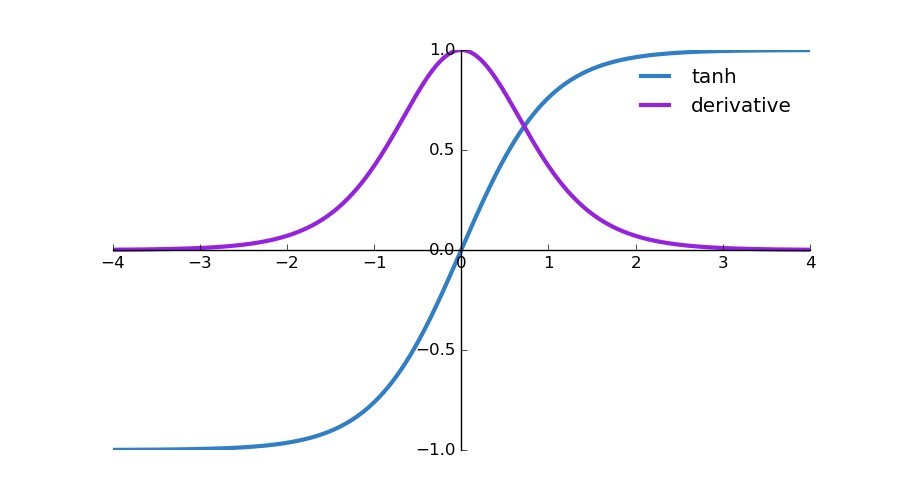
\includegraphics[width=15cm]{images/tanhfunc.jpg}
\caption{Đồ thị hàm số của hàm Tanh và đạo hàm của nó.}
\label{fig:tanhfunc}
\end{figure}

Một nhược điểm dễ nhận thấy là khi đầu vào có trị tuyệt đối lớn, đạo hàm của cả Sigmoid và Tanh tại điểm giá trị đó rất gần với 0.
Điều này đồng nghĩa với việc các hệ số tương ứng với đơn vị ẩn đang xét sẽ gần như không được thay đổi khi sử dụng công thức cập nhật theo thuật toán gradient khi tiến hành lan truyền ngược.
Hiện tượng này được gọi là hiện tượng biến mất gradient.

\section{Hàm ReLU (Rectified Linear Unit)}\label{sec:hamrelu}

Đây là hàm \cite{reluhinton} được sử dụng rộng rãi nhất trong các mô hình học sâu vì tính đơn giản của nó (xem hình \ref{fig:relufunc}).
Tuy đơn giản, nhưng không hề đồng nghĩa với ít hiệu quả.
Hàm kích hoạt này có công thức toán học là:
\begin{align}
    \text{ReLU}(x) = \mathcal{R}(x) = \max\left(0, x\right)
\end{align}

Một cách nôm na, ta có thể miêu tả hàm ReLU như sau:
\begin{itemize}
    \item Nếu đầu vào nhỏ hơn hoặc bằng 0, thì đầu ra là 0.
    \item Nếu đầu vào lớn hơn 0, thì đầu ra là chính nó, tức đầu ra đúng bằng đầu vào.
\end{itemize}

\begin{figure}[!h]
\captionsetup{width=0.8\textwidth}
\centering
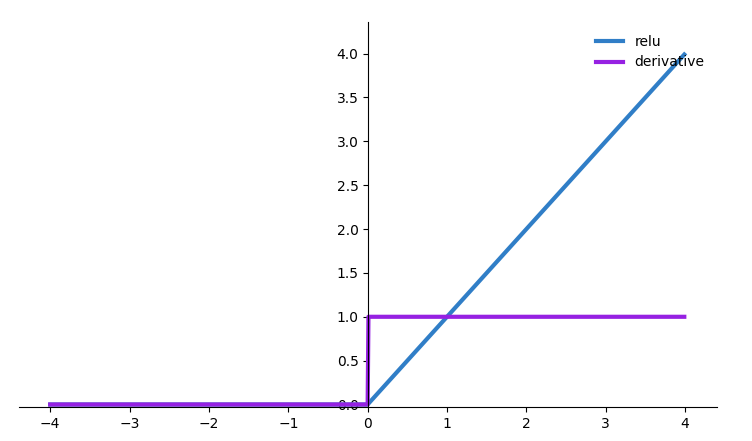
\includegraphics[width=15cm]{images/relufunc.PNG}
\caption{Đồ thị hàm số của hàm ReLU và đạo hàm của nó.}
\label{fig:relufunc}
\end{figure}

Ta có thể thấy, hàm ReLU thực sự rất đơn giản trong tính toán.
Nhìn vào tưởng chừng không khác mấy so với một hàm tuyến tính thông thường.
Hay thay, điều đơn giản này lại khắc phục được hiện tượng biến mất gradient mà hàm Sigmoid và Tanh mắc phải.
Để có thể thấy rõ điều đó, ta sẽ xem xét đạo hàm của hàm ReLU.
Hiển nhiên, ta không khó để ta tính được:
\begin{align}
    \dfrac{\text{d}\mathcal{R}}{\text{d}x} = \max\left(\text{sgn}\left(x\right)\right) = \begin{cases}1, x > 0\\0, x \le 0\end{cases}
\end{align}

Cũng như chính hàm ReLU, đạo hàm của nó cũng hết sức đơn giản:
\begin{itemize}
    \item Nếu đầu vào nhỏ hơn hoặc bằng 0, thì đầu ra là 0.
    \item Nếu đầu vào lớn hơn 0, thì đầu ra là 1.
\end{itemize}

Vậy nên sẽ không xuất hiện chuyện khi đầu vào quá lớn, đạo hàm tại giá trị đó sẽ rất gần 0, khiến cho việc cập nhật giá trị tham số mô hình diễn ra chậm.
ReLU được chứng minh là đã giúp việc huấn luyện mạng nơ-ron đa tầng nhanh hơn rất nhiều so với lại hàm Tanh.
\vspace{5pt}

Nhưng hàm này lại gây ra một trở ngại khác, chính là chết ReLU.
Mọi đầu vào nhỏ hơn hoặc bằng 0 đều sẽ được đưa về 0.
Chuyện gì sẽ xảy ra khi ta có nhiều đầu vào nhỏ hơn 0?
Hiển nhiên là kết quả tệ và thậm chí là tệ hơn so với biến mất gradient, khi giá trị tham số sẽ không có cách nào thay đổi và mãi như vậy do đạo hàm của những giá trị đầu vào này đều là giá trị 0.
Một số chứng minh thực nghiệm cho thấy, việc này có thể được khắc phục bằng cách tăng số lượng đơn vị ẩn \cite{activationfunctionandrew}.
Tuy nhiên, việc này cần phải cẩn thận khi Lu Lu \cite{Lu_2020} đã chứng minh lý thuyết được rằng một mạng học sâu với hàm kích hoạt ReLU sẽ chết khi độ sâu lên đến vô hạn.
\vspace{5pt}

Ưu điểm dễ dàng nhận ra của RELU đó chính là việc tính toán đơn giản, giúp cho chi phí tính toán sẽ đơn giản hơn những hàm sử dụng hàm mũ.
Đồng thời hàm này cũng khắc phục được hiện tượng biến mất gradient.
Tuy thế, phần âm đưa hết về 0 của hàm lại gây nên hiện tượng chết ReLU.

Theo kinh nghiệm của những kỹ sư đi trước, khi xây dựng một mạng nơ-ron đa tầng, hàm kích hoạt ReLU nên được thử đầu tiên, vì nó nhanh cho kết quả và thường hiệu quả trong nhiều trường hợp.

\section{Hàm Leaky ReLU}\label{sec:hamleakyrelu}

Đây là một biến thể của ReLU \cite{leakyandrew} mà có khả năng khắc phục hiện hượng chết ReLU.
Công thức toán học miêu tả hàm này như sau:
\begin{align}
    \text{Leaky ReLU}(x) = \mathcal{R}_L(x) = \begin{cases}x, &x > 0\\\alpha x, &x \le 0\end{cases}; \alpha \in \left(0, 1\right)
\end{align}

\begin{figure}[!h]
\captionsetup{width=0.8\textwidth}
\centering
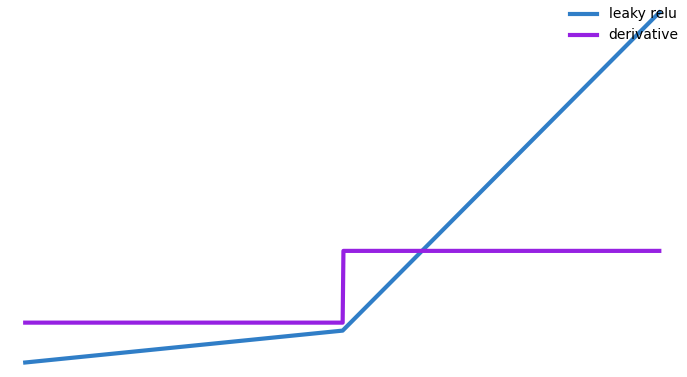
\includegraphics[width=15cm]{images/lrelu.PNG}
\caption{Đồ thị hàm số của hàm Leaky ReLU ($\alpha = 0.1$) và đạo hàm của nó.}
\label{fig:lrelu}
\end{figure}

Nửa khoảng giá trị $\left(0, +\infty\right)$, hai hàm ReLU và Leaky ReLU hoàn toàn giống nhau.
Duy chỉ phần nửa đoạn $\left(-\infty, 0\right]$, hàm Leaky ReLU đã có một chút sự thay đổi thay vì chỉ là giá trị 0 như ReLU.
Bây giờ, những giá trị âm sẽ có giá trị là $\alpha x$ thay vì giá trị $0$.
Đạo hàm của Leaky ReLU cũng vì thế mà sẽ là:
\begin{align}
    \dfrac{\text{d}\mathcal{R}_L}{\text{d}x} =  \begin{cases}1, x > 0\\\alpha, x \le 0\end{cases}
\end{align}

Nhờ như vậy, những đầu vào nhỏ hơn 0 bây giờ sẽ không bị đưa hết về 0 mà sẽ là $\alpha$.
Điều này có nghĩa là, hiện tượng chết ReLU đã được xử lý.
\vspace{5pt}

Việc lựa chọn giá trị $\alpha$ cho thực sự hiệu quả cũng là một vấn đề không hề đươn giản.
Nếu giá trị $\alpha = 0$, Leaky ReLU chính là ReLU.
Còn nếu $\alpha = 1$, thì Leaky ReLU sẽ trở thành một hàm tuyến tính, nên không ai sử dụng Leaky ReLU với $\alpha = 1$.
Thông thường, $\alpha$ sẽ được chọn là 0.01, tức 1 phần 100.
Cũng có một số mô hình chọn giá trị $\alpha$ lớn hơn một chút, khoảng từ 0.1 tới 0.3.
Đã có nhiều cải thiện được đề xuất cho Leaky ReLU và cũng đã có những kết quả khả quan trên một số thực nghiệm.
Có thể liệt kê qua như việc học hệ số $\alpha$ này trong quá trình huấn luyện với hàm đề xuất là PReLU (Parametric Rectified Linear Unit).
Hoặc là ngẫu nhiên chọn hệ số $\alpha$ dựa vào một biến ngẫu nhiên theo một phân phối đều - RReLU (Randomized Leaky Rectified Linear Unit).
\vspace{5pt}

Có thể nói, Leaky ReLU đã thừa hưởng được những đặc điểm tốt của ReLU, ngoài ra còn khắc phục được hiện tượng chết ReLU của phiên bàn gốc.
Nhưng một điều khá rắc rối là việc chọn hệ số $\alpha$ cần phải được thực hiện một cách hợp lý, hoặc phải dùng thuật toán học, nếu không dễ gây tác dụng không đáng có.

\section{Hàm ELU (Exponential Linear Unit)}\label{sec:hamelu}

Cũng như Leaky ReLU, hàm ELU \cite{clevert2016fast} được đưa ra để khắc phục điểm yếu của ReLU.
Một hệ số $\alpha$ sẽ được chọn giống như cách chọn cho hàm Leaky ReLU, đôi khi sẽ là chọn bằng kinh nghiệm, và có lúc sẽ là học trong quá trình huấn luyện.
Nhưng ELU không còn giữ được tính đơn giản tính toán như Leaky ReLU hay ReLU tuy hình dáng không thay đổi nhiều (xem hình \ref{fig:elufunc}).
Công thức toán học của ELU có thể được biểu diễn như sau:
\begin{align}
    \text{ELU}(x) = \mathcal{E}(x) = \begin{cases}x, &x > 0\\\alpha\left(e^x - 1\right), &x \le 0\end{cases}; \alpha \in \left(0, 1\right)
\end{align}

Nếu đầu vào lớn hơn 0, đầu ra bằng đúng đầu vào.
Còn với những đầu vào bé hơn hoặc bằng 0, chúng ta sẽ có một giá trị chỉ là gần với 0.
Khác so với ReLU, khi ReLU sẽ đưa hết tất cả về 0.
Leaky ReLU thì sẽ đưa trị tuyệt đối của giá trị đó nhỏ lại theo hệ số $\alpha$.
Những thay đổi của ELU cũng không làm mất đi tính chất của những họ hàm LU, dùng để giải quyết biến mất gradient.
Nếu như vậy, thì ELU có tránh được việc chết ReLU như Leaky ReLU làm được?
Ta hãy cùng xem đạo hàm của ELU:
\begin{align}
    \dfrac{\text{d}\mathcal{E}}{\text{d}x} =  \begin{cases}1, &x > 0\\\alpha e^x, &x \le 0\end{cases} =  \begin{cases}1, &x > 0\\\alpha\left(e^x - 1\right) + \alpha, &x \le 0\end{cases} =  \begin{cases}1, &x > 0\\\mathcal{E}(x) + \alpha, &x \le 0\end{cases}\label{eqn:daohamelu}
\end{align}

Lý do ta nên biểu diễn đạo hàm phía âm của hàm ELU dưới dạng $\mathcal{E}(x) + \alpha$ thay vì $\alpha e^x$ (\ref{eqn:daohamelu}) là để tái sử dụng lại giá trị $\mathcal{E}(x)$ thay vì phải tính lại giá trị $e^x$.
\vspace{5pt}

\begin{figure}[!h]
\captionsetup{width=0.8\textwidth}
\centering
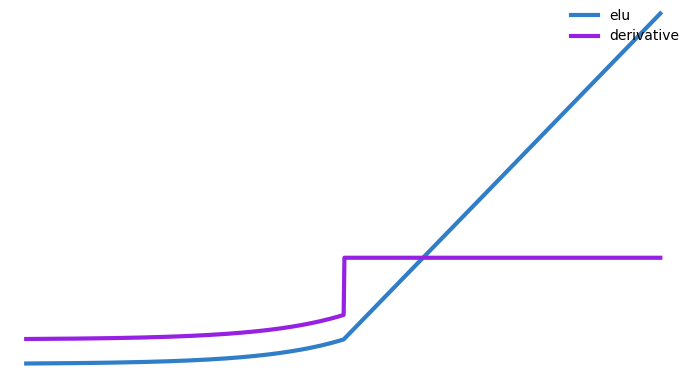
\includegraphics[width=15cm]{images/elufunc.PNG}
\caption{Đồ thị hàm số của hàm ELU ($\alpha = 0.3$) và đạo hàm của nó.}
\label{fig:elufunc}
\end{figure}

Trở lại với việc rằng liệu ELU có tránh được việc chết ReLU hay không, ta cần chú ý vào phần phía âm, tức đại lượng $\mathcal{E}(x) + \alpha$.
Rõ ràng rằng dù đầu vào của $\mathcal{E}(x)$ có âm như thế nào, thì giá trị nhận về cũng là một số âm gần với 0.
Khi cộng với một $\alpha$ lớn vừa phải, giá trị này sẽ có xu hướng lớn hơn 0 một tí, vừa đủ để thoát khỏi được hiện tượng chết ReLU.
Khác với Leaky ReLU, hàm ELU vẫn có thể có một vài đơn vị ẩn bị chết, tức không cập nhật được tham số nếu đầu vào rất âm.
Vì khi đó $\mathcal{E}(x)$ không còn quá gần 0, khi cộng vào với $\alpha$, sẽ có xu hướng rất sát với 0 như Sigmoid hoặc Tanh.
Hoặc có thể hiểu là do việc $x \rightarrow -\infty$ sẽ suy ra được $e^x \rightarrow 0$.
\vspace{5pt}

Hàm ELU cũng có được những ưu điểm của Leaky ReLU, tuy vậy việc tính toán lúc này sẽ phức tạp hơn một chút vì có đại lưỡng mũ.

\section{Hàm SELU (Scaled Exponential Linear Unit)}\label{sec:hamselu}

Hàm này \cite{klambauer2017selfnormalizing} là một trong những hàm khá mới (xem hình \ref{fig:selufunc}).
Việc cài đặt hàm này để sử dụng trong thực tiễn một cách hiệu quả cũng cần phải có nhiều công sức hơn so với các hàm đã giới thiệu.
Theo hướng dẫn, các trọng số cũng như bias của mạng cần phải được khởi tạo với LeCun Normal \cite{activationcasper}.
Trong trường hợp mạng có sử dụng kỹ thuật dropout, thì cần phải sử dụng Alpha Dropout.
Tác giả khi đề xuất hàm này, đã tính toán 2 giá trị quan trọng cho hàm này, chính là $\alpha$ và $\lambda$:
\begin{align}
    \alpha \approx 1.6732632423543772848170429916717 \label{eqn:selualpha}\\
    \lambda \approx 1.0507009873554804934193349852946 \label{eqn:selulambda}
\end{align}

Không giống như Leaky ReLU hay ELU, đây là những giá trị đã được các tác giả tính toán trước và áp dụng cho mọi mô hình.
Giống như cái tên của mình, đây là một hàm tỷ lệ với hàm ELU, chính xác là tỷ lệ với hệ số $\lambda$ (\ref{eqn:selulambda}):
\begin{align}
    \text{SELU}(x) = \mathcal{E}_S(x) = \lambda \begin{cases}x, &x > 0\\\alpha\left(e^x - 1\right), &x \le 0\end{cases}
\end{align}

Đạo hàm của SELU cũng không khác ELU là bao:
\begin{align}
    \dfrac{\text{d}\mathcal{E}_S}{\text{d}x} =  \lambda\dfrac{\text{d}\mathcal{E}}{\text{d}x} =  \begin{cases}1, &x > 0\\\mathcal{E}_S(x) + \alpha, &x \le 0\end{cases}\label{eqn:daohamselu}
\end{align}

\begin{figure}[!h]
\captionsetup{width=0.8\textwidth}
\centering
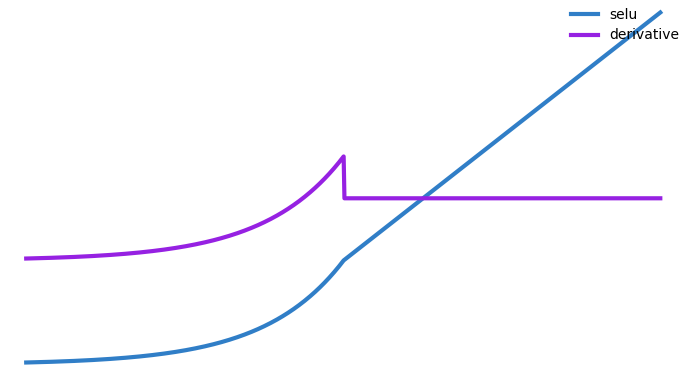
\includegraphics[width=15cm]{images/selufunc.PNG}
\caption{Đồ thị hàm số của hàm SELU và đạo hàm của nó.}
\label{fig:selufunc}
\end{figure}

Bây giờ, nếu đầu vào lớn hơn 0 thì giá trị đầu ra cần phải tỷ lệ theo một hệ số $\lambda$ thành là $\lambda x$ hay vì chính bằng $x$.
Phần miền nhỏ hơn hoặc bằng 0, tương tự một hàm ELU với giá trị $\alpha$ (\ref{eqn:selualpha}) đã chọn nhưng giá trị sẽ được tỷ lệ với $\lambda$.
\vspace{5pt}

Chọn một số $\alpha$ để cài đặt cho hàm ELU, và tỷ lệ với một hằng số $\lambda$, điều gì khiến hàm này trở nên đặc biệt?
Lý thuyết mà nói, hàm SELU là hàm có khả năng tự chuẩn hoá đầu ra nếu được cài đặt đúng như những gì đã yêu cầu.
Thay vì phải thêm một tầng chuẩn hoá đầu ra như một số các hàm khác, thì khi sử dụng SELU, bước chuẩn hoá này đã được hàm SELU tự động hoàn thành trong nội bộ.
Điều này giúp giảm thời gian huấn luyện của mô hình sử dụng hàm SELU.
\vspace{5pt}

Về bản chất, SELU cũng vẫn là một dạng tỷ lệ của ELU, nên cách nó khắc phục biến mất gradient và chết ReLU không khác gì ELU.
Nếu đúng như lý thuyết, thì SELU lợi thế hơn ELU ở điểm có khả năng tự chuẩn hoá, bớt cồng kềnh cho mạng sử dụng.

\section{Hàm GELU (Gaussian Error Linear Unit)}\label{sec:hamgelu}

Được sử dụng nhiều gần đây trong kiến trúc Transformers - Google's BERT và OpenAI's GPT-2.
Tuy ra đời cũng không phải là quá mới, khi 2016 đã được trình làng \cite{hendrycks2020gaussian}, nhưng mãi ít năm gần đây mới được chú ý tới.
Mô tả toán học của hàm này như sau:
\begin{align}
    \text{GELU}(x) = \mathcal{G}(x) = 0.5x\left\{1 + \tanh\left[\sqrt{\dfrac{2}{\pi}}\left(x + 0.044715x^3\right)\right]\right\}
\end{align}

\begin{figure}[!h]
\captionsetup{width=0.8\textwidth}
\centering
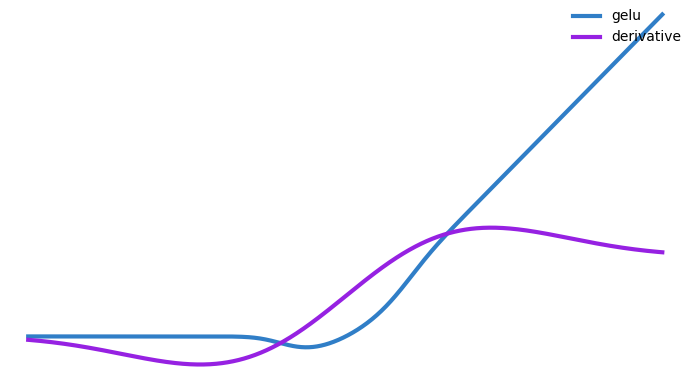
\includegraphics[width=15cm]{images/gelu.PNG}
\caption{Đồ thị hàm số của hàm GELU và đạo hàm của nó.}
\label{fig:gelufunc}
\end{figure}

Không có gì là giống với những hàm LU trước, khi bây giờ GELU là tổ hợp của nhiều hàm cộng lại: hàm Tanh, hàm đa thức, những hệ số vô tỉ.
Nếu để ý kĩ, hàm Tanh sẽ cho giá trị gần với 1 khi $x$ dương lớn, như vậy hàm GELU sẽ có giá trị đầu ra đúng gần bằng với đầu vào như là một hàm Linear Unit.
Muốn có cái nhìn chính xác của điều trên, ta quan sát những giá trị giới hạn và phép tương đương sau:
\begin{align}
\lim_{x \rightarrow +\infty}&\sqrt{\dfrac{2}{\pi}}\left(x + 0.044715x^3\right) = +\infty\\
\lim_{x \rightarrow +\infty}&0.5\left(1 + \tanh(x)\right) = 0.5\left(1 + 1\right) = 1\\
\mathcal{G}(x) \sim & 0.5x\left(1 + 1\right) = x, x \rightarrow +\infty
\end{align}

Trường hợp $x$ âm lớn, hàm Tanh sẽ cho ta giá trị gần với -1 khiến cho kết quả của hàm GELU có giá trị gần với 0.
Đại lượng âm vô cùng $x$ sẽ được khử với giá trị 0 của 1 + hàm Tanh.
Để hiểu rõ chỗ này, ta cần một số kiến thức giải tích cơ bản về chuỗi xấp xỉ tương đương Taylor-Maclaurin:
\begin{align}
    \frac{1}{1+x} = \sum_{n=0}^{\infty}(-1)^nx^n = 1 - x + x^2 - x^3 + \dots
\end{align}

Từ đó, ta có thể tương đương hàm Tanh như sau:
\begin{align}
    \tanh(x) &= \frac{e^x - e^{-x}}{e^x + e^{-x}} = \left(e^{2x} - 1\right).\dfrac{1}{e^{2x} + 1}\nonumber\\
    &= \left(e^{2x} - 1\right)\left(1 - e^{2x} + \dots\right) \sim -1 + e^{2x}, x \rightarrow -\infty \label{eqn:maclaurinoftanh}
\end{align}

Dựa vào \ref{eqn:maclaurinoftanh} vừa khai triển, ta suy ra được:
\begin{align}
    \tanh\left[\sqrt{\dfrac{2}{\pi}}\left(x + 0.044715x^3\right)\right] \sim \tanh\left(kx^3\right) \sim -1 + e^{2kx^3}, x \rightarrow -\infty
\end{align}

Theo đó, ta sẽ có được kết quả giới hạn:
\begin{align}
    \lim_{x \rightarrow -\infty}\mathcal{G}(x) &= \lim_{x \rightarrow -\infty}0.5x\left\{1 + \tanh\left[\sqrt{\dfrac{2}{\pi}}\left(x + 0.044715x^3\right)\right]\right\} \nonumber\\
    &= \lim_{x \rightarrow -\infty}0.5x\left\{1 - 1 + e^{2kx^3}\right\} \nonumber\\
    &= \lim_{x \rightarrow -\infty}0.5xe^{2kx^3} \nonumber\\
    &= \lim_{x \rightarrow +\infty}-\dfrac{0.5x}{e^{2kx^3}}; e^{x} >> x, x \rightarrow +\infty \nonumber\\
    &= 0
\end{align}

Không quá gian nan để tìm ra đạo hàm của GELU, bằng đạo hàm của hàm hợp ta có:
\begin{align}
     \dfrac{\text{d}\mathcal{G}}{\text{d}x} = 0.5&\tanh\left(0.0356774x^3 + 0.797885x\right) \nonumber\\
     &+ \frac{0.0535161x^3+ 0.398942x}{\cosh^2\left(0.0356774x^3 + 0.797885x\right)} + 0.5
\end{align}

Trong đó, hàm Cosh được định nghĩa như sau:
\begin{align}
    \cosh(x) = \dfrac{e^x + e^{-x}}{2}    
\end{align}

Cosh là một vô cùng lớn khi $x \rightarrow \infty$, nên là:
\begin{align}
    \lim_{x \rightarrow \infty}\dfrac{x^3}{\cosh(x^3)} &= 0\\
    \Rightarrow \dfrac{\text{d}\mathcal{G}}{\text{d}x} \sim 0.5\tanh(x^3) + 0.5 &\sim 0.5 + 0.5 = 1, x \rightarrow +\infty\\
    \Rightarrow \dfrac{\text{d}\mathcal{G}}{\text{d}x} \sim 0.5\tanh(x^3) + 0.5 &\sim -0.5 + 0.5 = 0, x \rightarrow -\infty
\end{align}

Nhìn sơ qua thì có vẻ công thức của GELU và đạo hàm của nó khá phức tạp, tuy nhiên khi được biểu diễn đồ thị lại là có hình ảnh cong mượt mà khá đẹp (xem hình \ref{fig:gelufunc}).
Điều này khác với những ReLU, Leaky ReLU, ELU hay SELU khi đồ thị hàm số bị gãy và đạo hàm không được liên tục (đạo hàm của ELU chỉ liên tục khi và chỉ khi $\alpha = 1$).
\vspace{5pt}

Tuy đã được đề xuất từ lâu, nhưng cũng như SELU, nghiên cứu về hiệu xuất hàm này trong thực tiễn vẫn chưa nhiều nên cần nhiều thực nghiểm để đưa ra kiểm chứng.

\section{Hàm Swish}\label{sec:hamswish}

\begin{figure}[!h]
\captionsetup{width=0.8\textwidth}
\centering
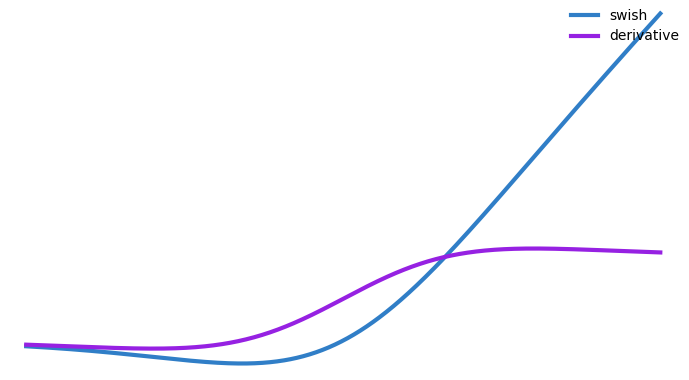
\includegraphics[width=15cm]{images/swish.PNG}
\caption{Đồ thị hàm số của hàm Swish ($\beta = 1$) và đạo hàm của nó.}
\label{fig:swishfunc}
\end{figure}

Không kinh khủng như GELU, Swish \cite{ramachandran2017searching} có công thức đơn giản hơn khi là một hàm tuyến tính bội với một hàm Sigmoid.
Đó cũng là lí do mà hàm này còn có cái tên khác là SiLU (Sigmoid Linear Unit):
\begin{align}
    \text{Swish}(x) = \mathcal{S}(x) = x\sigma(\beta x) = \dfrac{x}{1 + e^{-\beta x}}; \beta \in \mathbb{R}
\end{align}

Giống với các hàm LU khác (trừ Leaky ReLU), Swish không bị chặn trên nhưng lại bị chặn dưới.
Swish có hình dạng khá giống với GELU khi nó rất mượt mà không gãy và trông còn có vẻ mượt hơn (Xem hình \ref{fig:swishfunc}).
\vspace{5pt}

Có 2 trường hợp đặc biệt của hệ số $\beta$.
Với $\beta$ được chọn là $0$, hàm Swish gần giống như một hàm tuyến tính vì $\sigma(0x) = 0.5$.
Nếu $\beta \rightarrow \infty$, hàm Swish giờ đây trở thành một hàm ReLU do $\displaystyle \lim_{\beta \rightarrow -\infty}\sigma(\beta x) = 0, \lim_{\beta \rightarrow +\infty}\sigma(\beta x) = 1$.
Swish nằm giữa 2 thái cực là tuyến tính và ReLU biến thiên nhờ vào hệ số $\beta$.
\vspace{5pt}

Đạo hàm của hàm Swish tính được theo đạo hàm hàm hợp như sau:
\begin{align}
    \dfrac{\text{d}\mathcal{S}}{\text{d}x} &= \sigma\left(\beta x\right) + x.\beta\sigma\left(\beta x\right)\left(1 - \sigma\left(\beta x\right)\right) \nonumber\\
    &= \sigma\left(\beta x\right) + \beta x\sigma\left(\beta x\right) - \beta x \sigma^2\left(\beta x\right) \nonumber\\
    &= \beta x\sigma\left(\beta x\right) + \sigma\left(\beta x\right) - \beta x \sigma^2\left(\beta x\right) \nonumber\\
    &= \beta \mathcal{S}(x) + \sigma\left(\beta x\right)\left(1 - \beta \mathcal{S}(x)\right)
\end{align}

Đạo hàm của Swish có hình dáng gần giống với GELU và liên tục trên toàn miền (Xem hình \ref{fig:swishfunc}).
Về mặt lý thuyết, có vẻ Swish khá tương tự với GELU và cũng chưa có nhiều thực nghiệm trên các mô hình khác nhau của hàm này nên cũng chưa thể đưa ra nhận xét nào quá đặc biệt.

\section{Thông tin về các hàm kích hoạt được thực nghiệm}\label{sec:thongtincachamthucnghiem}

Trong các phần thực nghiệm sau, những hàm được đem vào những mô hình để đánh giá là Sigmoid, Tanh ($\tanh$), ReLU ($\mathcal{R}$), Leaky ReLU - sẽ được gọi tắt là Leaky ($\mathcal{R}_L (\alpha = 0.2)$), ELU ($\mathcal{E} (\alpha = 1)$), SELU ($\mathcal{E}_S = \lambda \mathcal{E}$), GELU ($\mathcal{G}$) và cuối cùng là Swish ($\mathcal{S} (\alpha = 1)$).